\section{Introduzione al problema}

%=======================================================================

\begin{frame}{Obiettivi del lavoro di tirocinio e tecnologie utilizzate}

\begin{columns}

\begin{column}{0.5\textwidth}

\begin{itemize}[<+->]
    \item Raccolta di (1) \textbf{tempi di esecuzione} e (2) \textbf{spazio utilizzato} degli algoritmi lightweight proposti nella famiglia ASCON
    \item \textbf{Analisi dei dati raccolti} per mostrare quali algoritmi sono i migliori e, per ogni algoritmo, quali implementazioni sono le migliori
\end{itemize}

\end{column}

\begin{column}{0.5\textwidth}
    
\begin{itemize}[<+->]
    \item[] 
\includegraphics[height=0.15\textwidth]{images/introduction/board.png} \vspace{0.5cm}
    \item[] 
\includegraphics[height=0.15\textwidth]{images/introduction/automation.png} \vspace{0.5cm}
    \item[] 
\includegraphics[height=0.15\textwidth]{images/introduction/plot.png}
\end{itemize}

\end{column}

\end{columns}

\end{frame}

%=======================================================================

\begin{frame}{Dispositivi utilizzati}

\begin{figure}
    \centering
    \begin{subfigure}[m]{0.30\textwidth}
        \centering
        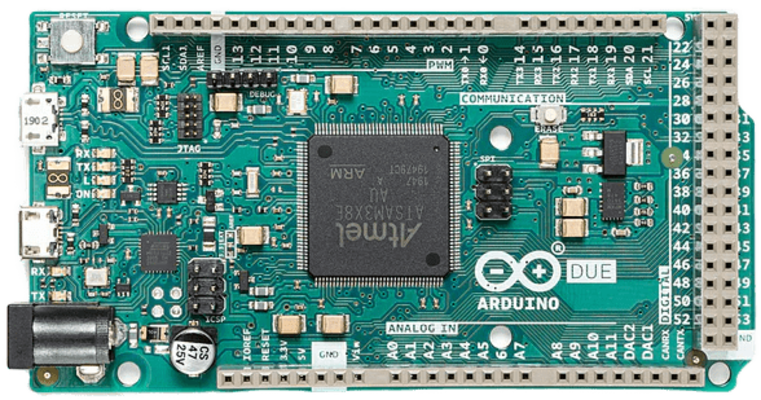
\includegraphics[height=0.49\textwidth]{images/introduction/arduino.png}
        \subcaption{Arduino Due.}
    \end{subfigure}
    \hfill \hfill \hfill
    \begin{subfigure}[m]{0.36\textwidth}
        \centering
        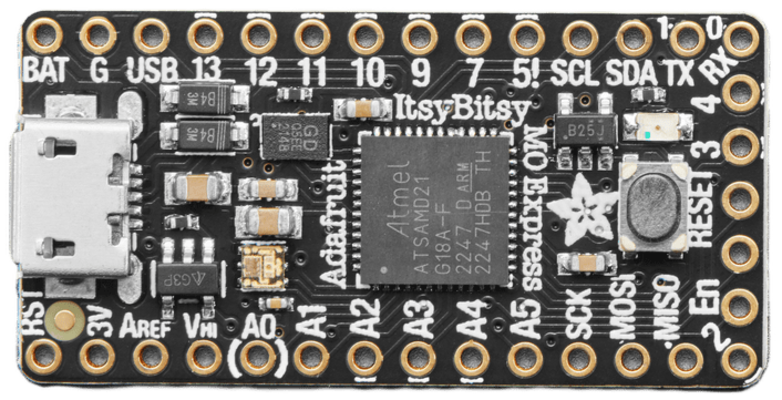
\includegraphics[height=0.40\textwidth]{images/introduction/adafruit.png}
        \subcaption{Adafruit ItsyBitsy M0 Express.}
    \end{subfigure}
    \hfill
    \begin{subfigure}[m]{0.30\textwidth}
    \centering
        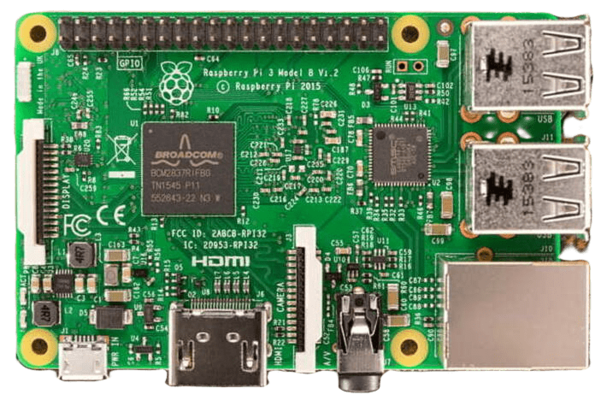
\includegraphics[height=0.48\textwidth]{images/introduction/raspberry.png}
        \subcaption{Raspberry Pi 3 Model B.}
    \end{subfigure}
\end{figure}

\end{frame}

%=======================================================================

\begin{frame}{Workflow}

\begin{center}
    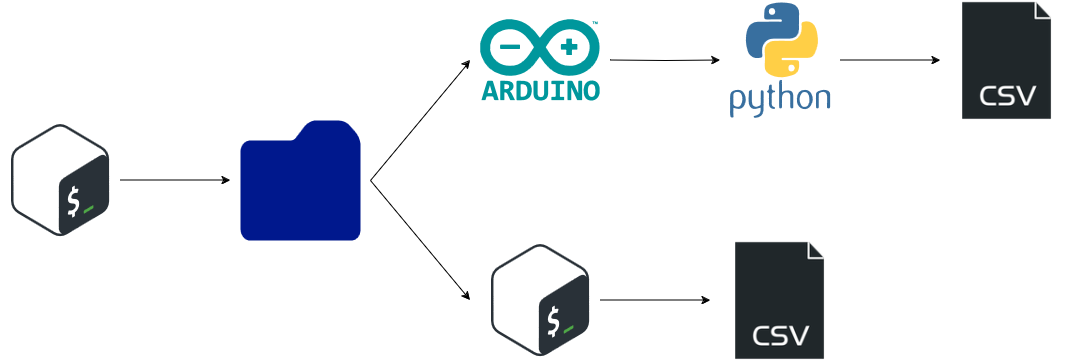
\includegraphics[height=0.30\textwidth]{images/introduction/workflow.png}
\end{center}

\end{frame}
